\documentclass[a4paper]{article}
\usepackage[pdftex]{graphicx}
\usepackage{anysize}
\marginsize{3cm}{3cm}{3cm}{3cm}
\linespread{1.2}
\usepackage[utf8]{inputenc}
\usepackage[T1]{fontenc}       
\usepackage[swedish]{babel}      
\usepackage{epstopdf}     % För svensk avstavning och svenska
\usepackage[osf]{mathpazo} % Palatino with smallcaps and oldstyle numbers
\usepackage[scaled]{helvet}
\usepackage{float}
\restylefloat{table}
\usepackage{etoolbox}

\newcommand\getcurrentref[1]{%
 \ifnumequal{\value{#1}}{0}
  {??}
  {\the\value{#1}}%
}  
\newcommand\requirement[2]{
	\numberedrow{Krav}{#1}{#2}
}
\newcommand\scenario[2] {
	\numberedrow{Scenario}{#1}{#2}
}
\newcommand\numberedrow[3]{
	\noindent
	\textbf{#1 \getcurrentref{section}.\getcurrentref{subsection}.#2.} #3
	
}

\usepackage{fancyhdr}
\fancyhf{}
\fancyhead[L]{Ansvarig: SG}

\fancyhead[R]{Datum: \today | Version: 0.18 | Dokumentnummer: PUSS144401}


\title{SRS - Software Requirements Specification: NewPussSystem}                  	
\author{Systemarkitektgruppen \\ Lars Gustafsson | Martin Lichota | Marcel Tovar Rascon}
\date{}

\begin{document}

\maketitle
\thispagestyle{fancy}
\tableofcontents
\newpage

\section*{Dokumenthistorik}

\begin{tabular}{ l l l p{8.5cm} }
Ver. & Datum & Ansv. & Beskrivning \\\hline
0.1 & 8 september 2014 & SG & Struktur för dokumentet\\
0.2 & 10 september 2014 & SG & Lägga till krav från UG\\
0.3 & 11 september 2014 & SG & Revidera krav samt ändra struktur\\
0.4 & 12 september 2014 & SG & Lade till nya samt reviderade krav\\
0.5 & 12 september 2014 & SG & Lade till nya samt reviderade krav\\
0.6 & 12 september 2014 & SG & Lade till nya samt reviderade krav\\
0.7 & 12 september 2014 & SG & Lade till nya samt reviderade krav\\
0.8 & 12 september 2014 & SG & Lade till nya samt reviderade krav\\
0.9 & 12 september 2014 & SG & Reviderade krav samt lade till scenarion\\
0.10 & 13 september 2014 & SG & Skapade scenarion för projektledning.\\
0.11 & 13 september 2014 & SG & Skapade scenarion för tidrapportmall och lade till krav.\\
0.12 & 14 september 2014 & SG & Administration och tidrapportering är klart.\\
0.13 & 14 september 2014 & SG & Lade till kontextdiagram samt uppdaterade krav under områdena projektledning, kvalitet och projekt.\\
0.14 & 15 september 2014 & SG & 

Uppdaterat efter granskningsprotokoll från TG, UG, och intern gransking i SG.
Uppdaterat formuleringar, kapitel 3.2 och 4. 
Uppdaterat krav, kapitel 6.1, 6.2, 6.3, 6.4, 6.5.
Lagt till nya krav, kapitel 6.3, 6.4, 6.5.
Uppdaterat scenario, kapitel 6.6. \\
0.15 & 16 september 2014 & SG & Uppdaterade design och lade till formulering, kapitel 4.
Lade till krav, kapitel 6.3.
Uppdaterade krav, kapitel 6.6, 7.2.\\
0.16 & 16 september 2014 & SG & Tog bort reduntant krav, kapitel 6.3.
Lade till krav, kapitel 6.3\\
0.17 & 16 september 2014 & SG & Ändrat krav 6.3.18, 6.3.19, scenario 6.4.4, scenario 6.4.1 och scenario 6.4.3. Lagt till krav 6.4.21, 6.4.22 och scenario 6.4.5.\\
0.18 & 21 september 2014 & SG & Större omstrukturering efter formell granskning.

\\
\end{tabular}
\section{Inledning}       
Dokumentet beskriver kraven för NewPussSystem, ett tidrapportingssystem för projekt som diverse användare kan logga in på.

\section{Referensdokument}
\begin{enumerate}
\item SRS - Software Requirements Specification: BaseBlockSystem (Dokumentnummer PUSS12002, version 1.0)
\end{enumerate}
\section{Bakgrund och mål}   
\subsection{Huvudmål}
Huvudmålet är att tillhandhålla ett system där olika användare, såsom projektledare och övriga projektmedlemmar, skall kunna tidrapportera och loggföra det fortgående arbetet i sitt projekt. 

\subsection{Aktörer och deras mål}
\label{bom-aktorer}
Följande aktörer kommer att använda systemet:
\begin{itemize}
\item [] \textbf{Vanlig användare} En vanlig användare är en person med ett konto i systemet som ännu inte har blivigt tilldelad ett projekt.
\item [] \textbf{Projektmedlem(t1,t2,t3)} En vanlig användare kan tilldelas rollen som projektmedlem. Denne kan tidrapportera och har även tillgång till historik rörande den egna samt gruppens totala tidrapportering. T1, t2, och t3 indikerar tre olika projektmedlemsroller, en användare blir tilldelad en av dessa i samband med att den blir medlem i ett projekt.
\item [] \textbf{Projektledare} En användare kan tilldelas rollen som projektledare vilket ger den administrativa rättigheter för ett givet projekt. En projektledare kan tillsätta vanliga användare en projektmedlemsroll. Utöver sina rättigheter som projektledare har den all funktionallitet som en projektmedlem besitter.
\item [] \textbf{Administratör} En administratör är en och endast en användare som har befogenheter att lägga till och ta bort andra användare. Administratören tillsätter även projektledare och skapar projektgrupper. Administratören kan inte deltaga i en projektgrupp men har utöver detta samma priviligerade rättigheter som projektledare coh projektmedlem.
\end{itemize}
\section{Terminologi}
\label{terminologi}
Här följer ord och uttryck som används i rapporten och är till för att öka förståelsen.
\begin{itemize}
\item []\textbf{Användarnamn:} Unik indentifikationsfras för att representera en användare i systemet..
\item []\textbf{Lösenord:} Hemlig fras endast känd för var unik användare samt systemet så användaren kan påvisa sin identitet.
\item []\textbf{Logga:} in Då en användare identifierar sig mot systemet med användarnamn och lösenord, om systemet godkänner identifieringen loggar användaren in.
\item []\textbf{Inloggad:} En användare som har loggat in är inloggad.
\item []\textbf{Användarstatus:} En indikation på var användare som avgör hur vida den får logga in eller ej.
\item []\textbf{Projektgrupp:} En grupp bestående av projektmedlemmar och projektledare.
\item []\textbf{Tidrapport:} En rapport som innehåller arbetsbelasting för en användare under en fix tidperiod bundet till en specefik projektgrupp.
\item []\textbf{Huvudsida:} Med huvudsida avses den första vyn som användaren blir dirigerad till direkt efter inloggning. 
\item []\textbf{Användarlista:} En lista med alla användarnamn och lösenord som är sparade i databasen.
\item []\textbf{Aktivitetsruta:} Cellen där aktivitet (raden) och subaktivitet (kolumnen) möts.
\item []\textbf{Information:} Med information avses t.ex. användare, projekt eller tidrapporter.
\item []\textbf{FIFO:} Från engelskans first in first out. Teknik som fungerar på samma sätt som en kö. Den som kom först betjänas först.

\end{itemize}
\section{Kontextdiagram}
Kontextdiagram för NewPussSystem illustreras av Figur \ref{image_kontext}.

\begin{figure}[h!]
  \centering
    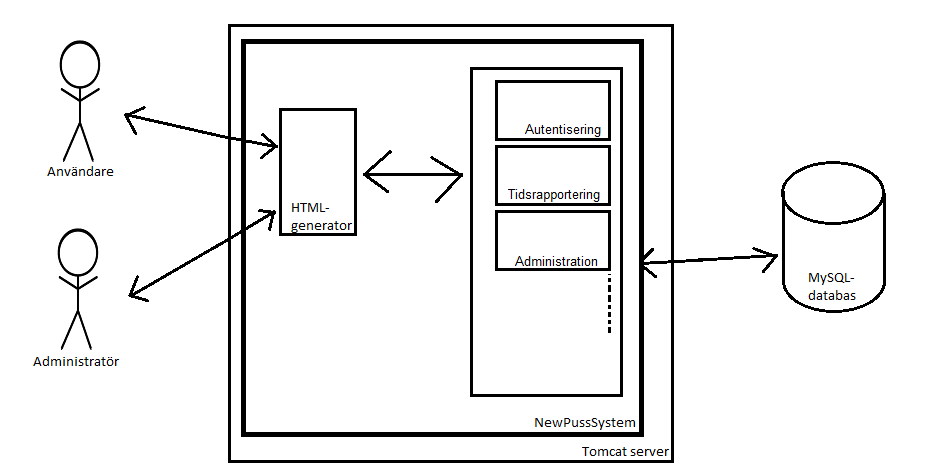
\includegraphics[width=0.75\textwidth]{context}
   \caption{Kontextdiagram för NewPussSystem.}
   \label{image_kontext}
\end{figure}

%  _  _______       __      __
% | |/ /  __ \     /\ \    / /
% | ' /| |__) |   /  \ \  / / 
% |  < |  _  /   / /\ \ \/ /  
% | . \| | \ \  / ____ \  /   
% |_|\_\_|  \_\/_/    \_\/    

\section{Funktionella krav}
	\subsection{Generella krav}
		\label{krav-funk-gen}
		\subsubsection*{Användare}
		\requirement{1}{Samtliga användare skall ha tillgång till följande funktionaliteter: tidrapportering, projektinformation, byta lösenord, samt utloggning.}
		
		\requirement{2}{Samtliga funktionaliter i krav 6.1.3 skall vara tillgängliga i menyn.}
		\requirement{3}{Menyn, oavsett typ av användare, skall vara tillgänglig på samtliga sidor som visas, för en inloggad användare, av systemet.}
		\requirement{4}{Krav 6.4.1 från Grundsystemet (Referensdokument 1) skall stödjas av systemet.}
		\requirement{5}{Det finns sammanlagt fem roller i systemet: administratör, projektledare, t1, t2, t3.}
		\requirement{6}{I varje projektgrupp får det finnas 1-2 projektledare (se krav 6.6.1) och de tre teamen, t1, t2 och t3 (se krav 6.1.13).}
		\subsubsection*{Projektledare}
		\requirement{7}{Varje projekt skall ha en eller två, och endast en eller två, användare som besitter rollen som projektledare.}
		\requirement{8}{Projektledarna har tillgång till projektadministrationsfunktionaliter. Det listas som ``projektadministration'' och finns tillgängligt för dem i menyn.}
		\subsubsection*{Administratör}
		\requirement{9}{Administratören kan ej deltaga i en projektgrupp. }
		\requirement{10}{Som inloggad administratör skall det vara möjligt att välja administrationsvyn på huvudsidan.}
		\subsubsection*{Data}
		\requirement{11}{Varje borttagning av information skall bekräftas av en dialogruta frågandes om man är säker. Om användaren väljer ``Ja'', tas informationen bort och användaren kommer tillbaka till en uppdaterad sida med informationen. Om ``Nej'' väljs, går användaren tillbaka till nuvarande sida.}


	\subsection{Autentisering}
		\label{krav-funk-aut}
		\subsubsection*{Övergripande}
			\requirement{1}{Ett användarkonto kan endast vara inloggat på en enhet åt gången.}			
			\requirement{2}{Om en användare försöker logga in med ett användarkonto som redan är inloggat på en annan enhet, kommer den nya inloggningen att genomföras medan den andra enheten loggas ut. }
			\requirement{3}{För varje användare kan loginstatus antingen vara inloggad eller inte inloggad.}
			\requirement{4}{Ett användarkonto kan endast vara inloggat på en enhet åt gången.}

			\requirement{5}{Krav 6.1.2 från Grundsystemet (Referensdokument 1) skall stödjas av systemet.}
			\requirement{6}{Krav 6.2.1 från Grundsystemet (Referensdokument 1) skall stödjas av systemet.}
			\requirement{7}{Krav 6.2.2 från Grundsystemet (Referensdokument 1) skall stödjas av systemet.}
			\requirement{8}{Krav 6.2.3 från Grundsystemet (Referensdokument 1) skall stödjas av systemet.}
			\requirement{9}{Krav 6.2.4 från Grundsystemet (Referensdokument 1) skall stödjas av systemet.}
\subsubsection*{Användare}
			\requirement{10}{Krav 6.1.3 från Grundsystemet (Referensdokument 1) skall stödjas av systemet.}
			\requirement{11}{Krav 6.1.4 från Grundsystemet (Referensdokument 1) skall stödjas av systemet.}
			\requirement{12}{Krav 6.1.5 från Grundsystemet (Referensdokument 1) skall stödjas av systemet.}
			\requirement{13}{Krav 6.1.8 från Grundsystemet (Referensdokument 1) skall stödjas av systemet.}
			\requirement{14}{Krav 6.1.9 från Grundsystemet (Referensdokument 1) skall stödjas av systemet.}


		\subsubsection*{Administratör}
			\requirement{15}{I administrationsvyn skall det vara möjligt att ta bort vilken användare som helst förutom administratören.}
			\requirement{16}{Om en administratör försöker lägga till en ny användare med ett användarnamn som strider mot krav 6.3.1-2 skall ett felmeddelande visas och användaren skall inte läggas till.}
			\requirement{17}{Scenario 6.4.1 skall stödjas av systemet.}
			\requirement{18}{Scenario 6.4.2 skall stödjas av systemet.}
			\requirement{19}{Scenario 6.4.3 skall stödjas av systemet.}
			\requirement{20}{Scenario 6.4.4 skall stödjas av systemet.}
			\requirement{21}{Scenario 6.4.5 skall stödjas av systemet.}
			\requirement{22}{Administratören skall kunna ta bort en tidrapportmall om den inte används av en projektgrupp (se krav 6.3.18).}
			
		\subsubsection*{Data}
			\requirement{23}{Krav 6.1.1 från Grundsystemet (Referensdokument 1) skall stödjas av systemet.}
			\requirement{24}{Krav 6.1.7 från Grundsystemet (Referensdokument 1) skall stödjas av systemet.}

		\subsubsection*{Ej inloggad}
			\requirement{25}{Krav 6.1.6 från Grundsystemet (Referensdokument 1) skall stödjas av systemet.}

	\subsection{Tidrapportering}
		\label{krav-funk-tid}	
		\subsubsection*{Projektmedlem}
			\requirement{1}{Projektmedlemmar skall kunna skapa, uppdatera och ta bort sina egna osignerade tidrapporter för de projekt de är medlemar i.}
			\requirement{2}{En projektmedlem kan bara se sina egna rapporter.}
			\requirement{3}{Projektmedlemmar ska inte kunna ta bort sina signerade rapporter.}
			\requirement{4}{Projektmedlemmar ska inte kunna redigera sina signerade rapporter.}
			\requirement{5}{Projektmedlemmar ska kunna föra in tidinformation enligt krav 6.3.4(???) och 6.3.12(???).}
			\requirement{6}{Scenario 6.5.1 skall stödjas av systemet.}
			\requirement{7}{Scenario 6.5.2 skall stödjas av systemet. }

		\subsubsection*{Projektledare}
			\requirement{8}{Projektledaren skall ha tillgång till samtliga projektmedlemmars tidrapporter i den projektgrupp den är projektledare för.}
			\requirement{9}{Projektledaren skall kunna godkänna ej tidigare godkända tidrapporter från projektmedlemmar i sin projektgrupp.}
			\requirement{10}{Projektledaren skall kunna ta tillbaka sitt godkännande från en tidigare godkänd gruppmedlems tidrapport, i sin projektgrupp.}
			\requirement{11}{Projektledaren skall kunna generera statistik över sitt projekt genom att summera tidrapporter per användare. Med summering menas att summera alla aktivitetsrutor till en ny tidrapport.}
			\requirement{12}{Projektledaren skall kunna generera statistik över sitt projekt genom att summera tidrapporter per roll. Med summering menas att summera alla aktivitetsrutor till en ny tidrapport.}
			\requirement{13}{Projektledaren skall kunna generera statistik över sitt projekt genom att summera tidrapporter per aktivitet. Med summering menas att samma aktivitet i alla tidrapporter läggs ihop i en ny tidrapport}
			\requirement{14}{Projektledaren skall kunna generera statistik över sitt projekt genom att summera tidrapporter per vecka. Med summering menas att summera alla aktivitetsrutor till en ny tidrapport.}
			\requirement{15}{Projektledaren skall kunna generera statistik över sitt projekt genom att summera tidrapporter per användare och aktivitet . Med summering menas att samma aktivitet i alla tidrapporter från samma användare läggs ihop i en ny tidrapport}
			\requirement{16}{Projektledaren skall kunna generera statistik över sitt projekt genom att summera tidrapporter per användare och vecka. Med summering menas att summera alla aktivitetsrutor till en ny tidrapport.}
			\requirement{17}{Projektledaren skall kunna generera statistik över sitt projekt genom att summera tidrapporter per roll och aktivitet. Med summering menas att samma aktivitet i alla tidrapporter från samma roll läggs ihop i en ny tidrapport}
			\requirement{18}{Projektledaren skall kunna generera statistik över sitt projekt genom att summera tidrapporter per roll och vecka Med summering menas att summera alla aktivitetsrutor till en ny tidrapport.}
			\requirement{19}{Projektledaren skall kunna generera statistik över sitt projekt genom att summera tidrapporter per aktivitet och vecka Med summering menas att samma aktivitet i alla tidrapporter från samma vecka läggs ihop i en ny tidrapport}
			\requirement{20}{Projektledaren ska kunna se sammanlagd arbetstid från valda tidrapporter}
			\requirement{21}{Projektledaren ska kunna se sammanlagd arbetstid för en vald aktivitet från valda tidrapporter}
			\requirement{22}{Projektledaren ska kunna se sammanlagd arbetstid för en vald subaktivitet från valda tidrapporter}
			\requirement{23}{Projektledaren ska kunna se hur ofta en vald aktivitet har utförts i valda tidrapporter}
			\requirement{24}{Projektledaren ska kunna se hur ofta en vald subaktivitet har utförts i valda tidrapporter}
			\requirement{25}{Projektledaren ska kunna se vilken aktivitet som har tagit mest tid.}
			\requirement{26}{Projektledaren ska kunna se vilken aktivitet som är vanligast}
			\requirement{27}{Projektledaren ska kunna se vilken vecka som har mest rapporterad tid.	}

		\subsubsection*{Data}
			\requirement{28}{Tidrapportering sker i antal minuter.}
			\requirement{29}{Namnet på tidrapportmallen ska bestå av 5 tecken, ascii (decimal) värden 48-57 och 97-122 är tillåtna.}
			\requirement{30}{Namnet på aktivitet och subaktivitet ska bestå av 3-5 tecken respektive 1 tecken, ascii (decimal) värden 48-57 och 97-122 är tillåtna.}

			\requirement{31}{Tidinformationen får innehålla 1-5 tecken per aktivitetsruta, ascii (decimal) värden 48-57.}
			\requirement{32}{Tidrapportmallarnas namn måste vara unika. }
 	 	 		
			\requirement{33}{Det skall gå att lagra 100 tidrapporter/användare. Efter uppnådd maxgräns skrivs de över enligt FIFO-principen.}
			\requirement{34}{Veckonumret får innehålla 1-2 tecken, ascii (decimal) värden 48-57 }
			\requirement{35}{En administratör skall kunna skapa tidrapportsmallar}
			\requirement{36}{Man skall kunna ange 1-20 stycken aktiviteter i en tidrapportsmall}
			\requirement{37}{Man skall kunna ange 1-20 stycken subaktiviteter i en tidrapportsmall }
			\requirement{38}{Antalet aktiviteter anger antalet rader som finns i tidrapportstabellen}
			\requirement{39}{Antalet subaktiviteter anger antalet kolumner som finns i tidrapportstabellen	}
			\requirement{40}{En tidrapport skall innehålla information om användarnamn}
			\requirement{41}{En tidrapport skall innehålla information om projektgruppsnamn}
			\requirement{42}{En tidrapport skall innehålla information om datum}
			\requirement{43}{En tidrapport skall innehålla information om veckonummer}
			\requirement{44}{Det skall tydligt framgå om en tidrapport är signerad eller inte}
			\requirement{45}{Maximalt 20 mallar kan lagras samtidigt.}

			\requirement{46}{En tidrapportmall kan endast tas bort om den inte används av någon projektgrupp. }
			\requirement{47}{Det skall inte vara möjligt att ändra tidrapportmallens utformning efter att den har skapats.}
			\requirement{48}{Nygenererade tidrapporter är alltid osignerade.}

			
			\requirement{49}{Tidrapportens grundmall skall innehålla information om användarnamn, projektgruppsnamn, datum och veckonummer. Det skall även tydligt framgå om den är signerad eller ej.}
			\requirement{50}{Grundmallen för tidrapporterna genereras automatiskt av systemet.}


	\subsection{Administration}
		\label{krav-funk-admin}
		\subsubsection*{Övergripande}
			\requirement{1}{Krav 6.3.3 från Grundsystemet (Referensdokument 1) skall stödjas av systemet.}		
			\requirement{2}{Krav 6.3.4 från Grundsystemet (Referensdokument 1) skall stödjas av systemet.}
			
		\subsubsection*{Projektledare}
			\requirement{3}{Projektledaren skall kunna tilldela roller till projektmedlemmarna i sin projektgrupp.}


			\requirement{4}{Projektledaren skall kunna lista alla ej godkända tidrapporter.}
			\requirement{5}{Projektledaren skall kunna lista alla godkända tidrapporter.}
			\requirement{6}{Scenario 6.6.1 skall stödjas av systemet.}
			\requirement{7}{Scenario 6.6.2 skall stödjas av systemet.}
			\requirement{8}{Scenario 6.6.3 skall stödjas av systemet.}
			\requirement{9}{Projektledaren skall kunna lista projektets alla tidrapporter och sortera dom efter följande attribut i både stigande och fallande ordning; Användare, vecka, och huruvida rapporten är godkänd eller ej.}
			\requirement{10}{Scenario 6.6.4 skall stödjas av systemet. }

		\subsubsection*{Administratör}
			\requirement{11}{Administrationsfunktionaliteter avser även projektadministration och därmed har administratörer, utöver sina priviligerade rättigheter, även projektledarnas befogenheter.		}
			\requirement{12}{Endast administratören skall kunna skapa projektgrupper i systemet.}
			\requirement{13}{Endast administratören skall kunna lägga till eller ta bort projektledare i en projektgrupp.}
			\requirement{14}{Endast administratören skall kunna ta bort projektgrupper ur systemet.}
			\requirement{15}{Scenario 6.4.1 skall stödjas av systemet.}
			\requirement{16}{Scenario 6.4.2 skall stödjas av systemet.}
			\requirement{17}{Scenario 6.4.3 skall stödjas av systemet.}
			\requirement{18}{Scenario 6.4.4 skall stödjas av systemet.}
			\requirement{19}{Scenario 6.4.5 skall stödjas av systemet.}
			\requirement{20}{Krav 6.3.1 från Grundsystemet (Referensdokument 1) skall stödjas av systemet.}
			\requirement{21}{Krav 6.3.5 från Grundsystemet (Referensdokument 1) skall stödjas av systemet.}
			\requirement{22}{Krav 6.3.6 från Grundsystemet (Referensdokument 1) skall stödjas av systemet.}
			\requirement{23}{Krav 6.3.7 från Grundsystemet (Referensdokument 1) har utgått och ersatt av krav 6.1.11}
			\requirement{24}{Krav 6.3.8 från Grundsystemet (Referensdokument 1) skall stödjas av systemet.}
			\requirement{25}{Krav 6.3.9 från Grundsystemet (Referensdokument 1) skall stödjas av systemet.}
			\requirement{26}{Krav 6.3.10 från Grundsystemet (Referensdokument 1) skall stödjas av systemet.}
			\requirement{27}{Krav 6.3.11 från Grundsystemet (Referensdokument 1) skall stödjas av systemet.		}
			\requirement{28}{Tidrapportens utseende, med avseende på vilka aktiviteter man kan föra in tidinformation i, bestäms av administratören innan projektgruppen har skapats. När projektet är skapat skall det inte gå att ändra tidrapportens utseende.}
		

		\subsubsection*{Data}
			\requirement{29}{Ett projektgruppsnamn ska bestå av 5-10 tecken, ascii (decimal) värden 48-57 och 97-122 är tillåtna.}
			\requirement{30}{Projektgruppsnamn måste vara unika. }
			\requirement{31}{Det får maximalt existera 5 stycken projektgrupper samtidigt.}
			\requirement{32}{En användare kan vara projektmedlem i fler än ett projektgrupp åt gången.}
			\requirement{33}{En projektgrupp skall bestå av 1-20 användare.}
			\requirement{34}{I varje projektgrupp kan det finnas upp till tre team, t1, t2 och t3.}
			\requirement{35}{I t1, t2 och t3 får det finnas 0-6 användare/projektgrupp, alltså sammanlagt 0-18 användare.}
			\requirement{36}{Krav 6.3.2 från Grundsystemet (Referensdokument 1) skall stödjas av systemet.}


\section{Kvalitetskrav}
	\subsection{Underhåll}
		\requirement{1}{Systemet skall vara väl dokumenterad så det underlättar vidareutvekling av systemet i framtiden.}
		\requirement{2}{Krav 7.1.1 från Grundsystemet (Referensdokument 1) skall stödjas av systemet.}
		\requirement{3}{Förståelse av Java, i nivå med vad som lärs ut i kursen EDA016, samt grundläggande kunskap av SQL skall räcka för att underhålla samt vidareutvekla systemet.}



	\subsection{Prestanda}
		\label{krav-kval-pres}
		\requirement{1}{Systemet skall klara av att få 20 stycken inloggningar under en tidperiod av 1 sekund, utan att bryta mot några andra kvalitetskrav.}
		\requirement{2}{Krav 7.2.1 från Grundsystemet (Referensdokument 1) skall stödjas av systemet.	}
		\requirement{3}{Maximalt 50 användare kan vara inloggade på systemet samtidigt.}

	\subsection{Användarvänlighet}
		\requirement{1}{Minst 7/10, på måfå utvalda Civilingenjörsstudenter, skall finna det lätt att använda systemet.}

\section{Projektkrav}
	\subsection{Utvecklingsmiljö}
	\requirement{1}{Krav 8.1.1 från Grundsystemet (Referensdokument 1) skall stödjas av systemet.}
	\requirement{2}{Krav 8.1.2 från Grundsystemet (Referensdokument 1) skall stödjas av systemet.}
	\requirement{3}{Krav 8.1.3 från Grundsystemet (Referensdokument 1) skall stödjas av systemet.}
	\requirement{4}{Systemet samt projekt- och produktdokumentation skall skrivas på svenska. Java- koden skall följa standarden som finns på http://www.geosoft.no/development/javastyle.html, alla variabelnamn skall vara skrivna på engelska.}




\end{document}